\documentclass[12pt, letterpaper]{article}
\usepackage{minutes}
\usepackage{background} %uncomment to create draft text

\newcommand{\blank}{\_\_\_\_\_\ }

\newcommand{\ousa}{Ontario Undergraduate Student Alliance}

\newcommand{\vpe}{Vice President, Education}
\newcommand{\vpof}{Vice President, Operations and Finance}
\newcommand{\vpi}{Vice President, Internal}
\newcommand{\vpsl}{Vice President, Student Life}
\newcommand{\pres}{President}

\newcommand{\antonio}{President Brieva}
\newcommand{\jill}{Vice President Knight}
\newcommand{\brian}{Vice President Schwan}
\newcommand{\andrew}{Vice President Clubine}
\newcommand{\aisha}{Aisha Shibli}
\newcommand{\tomson}{Councillor Tran}
\newcommand{\tristan}{Councillor Potter}
\newcommand{\rebecca}{Councillor George}
\newcommand{\stephanie}{Councillor Ye-Mowe}
\newcommand{\subham}{Councillor Altaf}
\newcommand{\ben}{Councillor Easton}
\newcommand{\alexander}{Councillor Ayre}
\newcommand{\jason}{Councillor Small}
\newcommand{\elizabeth}{Councillor O'Sullivan}
\newcommand{\andrew}{Councillor Mohan}
\newcommand{\seneca}{Councillor Velling}
\newcommand{\wenyu}{Councillor Xu}

\newcommand{\william}{William MacDonald}

\meetingDate{May 28, 2018} 
\meetingLocation{SLC MPR, University of Waterloo}
\speaker{\antonio}
\secretary{\jill}

\begin{document}

\hypersetup{} % setting up hyperlinks

\header{} % header macro with attendance as params

\section*{Attendance}

\begin{multicols}{2}[
        The following members were present:
    ]

\begin{itemize}
    \item Altaf, Subham
    \item Brieva, Antonio
    \item Clubine, Andrew
    \item Easton, Benjamin
    \item Eyre, Alexander
    \item George, Rebecca
    \item Knight, Jill
    \item Mohan, Andrew
    \item O'Sullivan, Elizabeth
    \item Potter, Tristan
    \item Schwan, Brian
    \item Shibli, Aisha
    \item Small, Jason
    \item Tran, Tomson
    \item Velling, Seneca*
    \item Xu, Wenyu*
    \item Ye-Mowe, Stephanie
\end{itemize}

\end{multicols}
* remote \\

\begin{multicols}{2}
    [
        The following members were absent:
    ]
\begin{itemize}
    \item Clarke, Antonio
    \item Goomer, Kanishk
    \item Jowhari, Nickta 
    \item Mills, Cameron
    \item Mistry, Harsh
    \item Simpson, Abigail
    \item Terzian, Hagop
\end{itemize}
\end{multicols}
* excused\\

\begin{multicols}{2}[
        The following gallery was present:
    ]
\begin{itemize}
    \item Kim, Ju Hyun     
    \item MacDonald, William
\end{itemize}
\end{multicols}

\noindent

\section*{Preliminaries}

\heading{Call to Order}
\begin{information}
    \call{12:55 PM}
\end{information}

\heading{Appointment of the Speaker}
\begin{motion}
    \birt Student's Council appoints \andrew\ as temporary speaker for the 
    current meeting.
    \movers{\brian}{\ben}

    \carries unanimously.
\end{motion}

\speaker{\andrew}

\heading{Appointment of the Secretary}
\begin{motion}
    \birt Student's Council appoints \blank as secretary, for the term 
    ending April 30, 2018.
    \movers{\brian}{\antonio}
    
    \brian\ nominates \tristan\, who accepts the nomination. There were no 
    other nominees.

    The motion now reads:

    \birt Student's Council appoints \tristan\ as secretary, for the term 
    ending April 30, 2018.

    \carries\ unanimously.
\end{motion}

\secretary{\tristan}

\heading{Appointment of the Assistant Secretary}
\begin{motion}
    \birt Student's Council appoints \blank as assistant secretary, for the
    term ending April 30, 2018. 
    \movers{\brian}{\tristan}

    \wenyu\ nominates themselves. There were no other nominees. 

    The motion now reads:

    \birt Student's Council appoints \wenyu\ as assistant secretary, for the
    term ending April 30, 2018. 

    \carries unanimously. 
\end{motion}

As \wenyu\ is participating remotely, they will assume their duties at the next
meeting. Until then, \jill\ continues as acting assistant secretary. 

\heading{Approval of the agenda}
\begin{motion}
    \birt Student's Council approves the agenda as presented. 
    \movers{\brian}{\jason}

    \brian\ updated an inacuracy in the agenda. The councillor appointment to
    Budget Committee is made by recommendation to the Board of Directors.

    \carries unanimously. 
\end{motion}

\section*{Executive Reports}

Please see the attached written reports for the full reports from the Executive
Board to Student's Council. 

All executive's spent this month preparing for their terms, including hiring 
their staff and creating their individual annual plans for the term.

\heading{Report of the \pres}
\begin{information}

    The \pres\ noted that construction on the expansion to the Student Life
    Centre and Physical Activites Complex had begun, and that all students had
    recieved an email detailing how they would be affected. A ground-breaking
    ceremony is being planned for June 19, 2017 and the \pres\ will be 
    co-hosting with President Bruce of the Graduate Students Association. 
    
    The \pres\ also touched on some of the plans they were making for the year,
    as well as the positive advocacy relationships that had already begun. 

    As an example, Premier Kathleen Wynne came to campus to promote the new 
    PharmaPlus plan. The \pres\ also took the opportunity to also discuss the 
    governments roll in preventing sexual violence on campus; a follow up 
    meeting was scheduled to discuss the matter in more depth.

    More locally, the \pres\ was invited to a police task force on sexual 
    violence and how it affects students. 

    Finally, the \pres\ highlighted that some work had begun on the new
    President's Advisory Commitee on Mental Health, and that Student's Council 
    could expect more updates at future meetings. 

\end{information}

\heading{Report of the \vpi}
\begin{information}

    The \vpi\ also made note of the work happening in the University related
    to student mental health, including that there would be plenty of 
    opportunities for Councillors to get their constituents active in the 
    discussion. 
    
    In addition, the \vpi\ is involved in a wellness committee that is 
    investigating how partners on campus are working towards a culture of 
    wellness on campus. The goal is to have all of the stakeholders working
    together in a unified direction. 
    
    In terms of student life,  the \vpi\ spent time learning more about the 
    clubs and services ecosystem, and has determined some termly goals for the 
    services as well as ensuring that the club support team has the 
    necessary resources to excel in their roles. 

    Finally, the \vpi\ will be investigating potential renovations to 
    the multi-faith prayer space to differentiate it from a classroom 
    and make it more accomodating.

    A councillor inquired about the Federation's plans to increase interaction
    with the student societies, and was informed that the \vpi\ is attending 
    the society executive meetings, organizing lunch and learns with the
    society executives, and increasing the role of the Committee of Presidents
    within their portfolio. 
    
\end{information}

\heading{Report of the \vpe}
\begin{information}

    The \vpe\ provided an update on the co-op fee review process that
    was promised as part of their platform. Meetings with the Director of Coop
    are proceeding and the terms of reference for the fee review committee are 
    being discussed.

    In addition to their university advocacy, the \vpe\ attended a conference 
    held by the \ousa\ and was elected President. They anticipate that this 
    will assist them in achieving the goals of the Federation in concert with 
    those of the \ousa.

    Finally, the \vpe\ shared their desire to improve the Federation's policy 
    framework with research and evidence to support existing policy, and
    they encouraged councillors to contact them to discuss any policy
    they felt the Federation was lacking. In response to a question from 
    Student's Council, the \vped\ also expressed that a large amount of the 
    Federation's policy is expired or expiring in the near future, and that
    councillors and their consituents could find the Federation's policies
    and their expiration dates online.

\end{information}

\heading{Report of the \vpof}
\begin{information}

    Beginning with the commercial services, the \vpof\ highlighted that there
    was an increase in traffic to Bomber and plans for a new menu. 
    As well, they announced that the selection of hot items at iNews had 
    increased, stocking three hot meals a day and Campus Bubble
    now serves chocolate ice cream and twist cones. 

    Internally, the new website encountered some unexpected issues
    with its backend but will be launched soon. 

    Finally, the \vpof\ drew attention to the recent government announcement
    on subsidized access to medication. 
    They are working closely with StudentCare to determine how the 
    Federation's health insurance plan will change with the new Pharmacare
    Plus program. A current lack of details about the
    plan is making it difficult to arrive at long-term sustainable decisions. 
    At the moment, fees haven't changed for the health and dental plan; until 
    more details are released the plan will operate as usual. 

\end{information}

\heading{Speaker's Report}
\begin{information}

    Given that no Speaker has been appointed, there was no formal report 
    submitted for this meeting; however, \printSpeaker\ highlighted the
    need for councillors to attend meetings and that council policy 
    stated that councillors may be removed after two un-excused absenses or
    four excused absenses. 

\end{information}

% \section*{Consent}
% \heading{Approval of the minutes}
% \begin{motion}
%     \birt Board approve the minutes from April \blank, 2017.
%     \movers{\tomson}{\abdullah}
%     \carries unanimously.
% \end{motion}

\section*{General Orders}
\heading{Election of Committees}
\begin{motion}
    \birt Council appoint members to the following committees. \begin{itemize}

        %% PPC
        \item \blank and \blank to fill the councillor seats on the Policy and 
            Procedures Committee.
            \begin{itemize}
                \item \tristan\ nominated himself.
                \item \seneca\ nominated himself.
            \end{itemize}

            There were no other nominees, \tristan\ and \seneca\ fill the 
            blanks.

        \item \blank and \blank to fill the at-large seats on the Policy and 
            Procedures Committee.

            There were no nominees. 

        %% CLAC
        \item \blank and \blank to fill the councillor seats on the Campus 
            Life Advisory Committee. 
            \begin{itemize}
                \item \tomson\ nominated himself.
                \item \alexander\ nominated himself.
            \end{itemize}

            There were no other nominees, \tomson\ and \alexander\ fill the
            blanks. 

        \item \blank and \blank to fill the at-large seats on the Campus 
            Life Advisory Committee. 

            There were no nominees. 

        %% IAC
        \item \blank and \blank to fill the councillor seats on the Internal
            Administration Committee.
            \begin{itemize}
                \item \tomson\ nominated himself.
                \item \alexander\ nominated himself.
                \item \subham\ nominated himself. 
            \end{itemize}

            \tomson\ withdrew his nomination. There were no other nominees,
            \alexander\ and \subham\ fill the blanks. 

        \item \blank and \blank to fill the at-large seats on the Internal
            Administration Committee.

            There were no nominees. 

        %% EAC
        \item \blank, \blank, and \blank to fill the councillor seats on the 
            Education Advisory Committee.
            \begin{itemize}
                \item \jason\ nominated himself.
                \item \ben\ nominated himself.
                \item \stephanie\ nominated herself.
                \item \alexander\ nominated himself. 
            \end{itemize}

            \alexander\ withdrew his nomination. There were no other nominees,
            \ben, \stephanie, and \jason\ fill the blanks. 

        \item \blank and \blank to fill the at-large seats on the 
            Education Advisory Committee.
            \begin{itemize}
                \item \tomson\ nominated himself.
                \item \william\ nominated himself.
            \end{itemize}

            There were no other nominees, \tomson\ and \william\ 
            fill the blanks. 

        %% PAC
        \item \blank and \blank to fill the councillor seats on the 
            Presidents Advisory Committee.
            \begin{itemize}
                \item \seneca\ nominated himself.
                \item \rebecca\ nominated herself.
            \end{itemize}

            There were no other nominees, \seneca\ and \rebecca\ fill the 
            blanks. 

        \item \blank and \blank to fill the at-large seats on the 
            Presidents Advisory Committee.

            There were no nominees.

        %% IFC
        \item \blank and \blank to fill the councillor seats on the 
            Internal Funding Committee.
            \begin{itemize}
                \item \ben\ nominated himself.
                \item \tomson\ nominated himself.
            \end{itemize}

            There were no other nominees, \ben\ and \tomson\ fill the 
            blanks. 

        \item \blank and \blank to fill the at-large seats on the 
            Internal Funding Committee.

            There were no nominees.

        %% GAAC
        \item \blank, \blank, and \blank to fill the councillor seats on the 
            Government Affairs Advisory Committee.
            \begin{itemize}
                \item \jason\ nominated himself.
                \item \stephanie\ nominated herself.
                \item \subham\ nominated himself.
                \item \ben\ nominated himself.
            \end{itemize}

            \subham\ withdrew his nomination. There were no other nominees,
            \jason, \stephanie, and \ben\ fill the blanks. 

        \item \blank and \blank to fill the at-large seats on the 
            Government Affairs Advisory Committee.

            There were no nominees.

        %% CSC
        \item \blank, \blank, and \blank to fill the councillor seats on the 
            Cooperative Student's Council.
            \begin{itemize}
                \item \subham\ nominated himself.
                \item \rebecca\ nominated herself.
                \item \seneca\ nominated himself.
                \item \elizabeth\ nominated herself.
                \item \jason\ nominated himself.
            \end{itemize}

            There were no other nominees; however, given that there were more
            nominees than available seats the appointment proceeded to a
            secret ballot. The Chair reviewed the terms of reference for the 
            committee and its existing membership, and each nominee was
            given a speaking turn. Councillors cast their ballots, and it was
            determined that \rebecca, \seneca, and \elizabeth\ fill the blanks. 

        \item \blank and \blank to fill the at-large seats on the 
            Cooperative Student's Council.
            \begin{itemize}
                \item \william\ nominated himself.
                \item \jason\ nominated himself.
            \end{itemize}

            There were no other nominees, \william\ and \jason\ 
            fill the blanks. 
    \end{itemize}
    \movers{\brian}{\jill}
    \carries unanimously.
\end{motion}

\begin{motion}
    \birt the ballots created in the election of councillors to the 
    Cooperative Student's Council be destroyed. 
    \movers{\brian}{\jill}
    \carries unanimously. 
\end{motion}

\heading{Councillor seat on the Budget Committee}
\begin{information}

    The \vpof\ informed Student's Council that the process for creating the 
    budget had started, and that there was a seat on the Budget Committee
    for an interested councillor. 

    \seneca\ and \wenyu\ expressed an interest in being considered for the 
    position, and the \vpof\ committed to bringing their names forward
    for consideration at the next meeting of the Board of Directors. 

\end{information}

\heading{Vacant at-large committee seats}
\begin{motion}
    \birt councillors may fill vacant at-large committee seats, subject to 
    ratification at the next council meeting. 
    \movers{\jason}{\ben}

    \carries unanimously.
\end{motion}

\heading{Appoint service coordinators}
\begin{motion}
    \birt Student's Council appoint the service coordinators for the Spring 2017 term. 
    \movers{\jill}{\brian}

    Student's Council was informed that the coordinators are selected by the 
    \vpi\ and then approved by Student's Council. This is because Student's
    Council has the ability to remove coordinators from their positions. 

    A councillor inquired about the turnover between spring terms, and the 
    \vpi\ responded that there were about six returning coordinators. 

    \birt the appointment is postponed until the next meeting of Student's
    Council.
    \movers{\antonio}{\ben}

    \carries unanimously. 
\end{motion}

\section*{New Business}

\heading{Next Meeting Date}
\begin{motion}
    \birt the next meeting of Student's Council occur on \blank and,
    \bifrt the chair will send out a poll to determine the July and August meeting
    dates. 
    \movers{\brian}{\jason}

    After a brief discussion, June 18, 2017 was proposed as a potential meeting
    date. No councillor expressed a conflict with this date. 

    \birt the blank be filled with June 18, 2017. 
    \movers{\brian}{\jason}
    \carries unanimously. 

    The motion now reads: 
    \birt the next meeting of Student's Council occur on June 18, 2017 and,
    \bifrt the chair will send out a poll to determine the July and August meeting
    dates. 

    \carries unanimously. 
\end{motion}

\heading{Reconsider the appointment of officers}
\begin{motion}
    \birt Student's Council reconsider the preliminary meeting motions on
    the appointment of the speaker and deputy speaker of Student's Council.
    \movers{\seneca}{\ben}
    \carries unanimously. 

    The following motion is on the table: 
    \birt Student's Council appoints \blank as speaker, for the term 
    ending April 30, 2018 and,
    \bifrt Student's Council appoints \blank as deputy speaker, for the term
    ending April 30, 2018.

    \seneca\ nominates \elizabeth\ as speaker. She accepts. 
    No other nominees, \elizabeth\ fills the blank for speaker. 

    \seneca\ nominates himself as Deupty Speaker. No other nomineees, 
    \seneca\ fills the blank for deputy speaker. 

    The motion now reads: 

    \birt Student's Council appoints \elizabeth\ as speaker, for the term 
    ending April 30, 2018 and,
    \bifrt Student's Council appoints \seneca\ as deputy speaker, for the term
    ending April 30, 2018.

    \carries unanimously.

\end{motion}

\section*{Adjournment}

\begin{motion}
    \birt Student's Council adjourns.
    
    With no other business the speaker adjourned the meeting at 2:07 PM. 
\end{motion}

\newpage
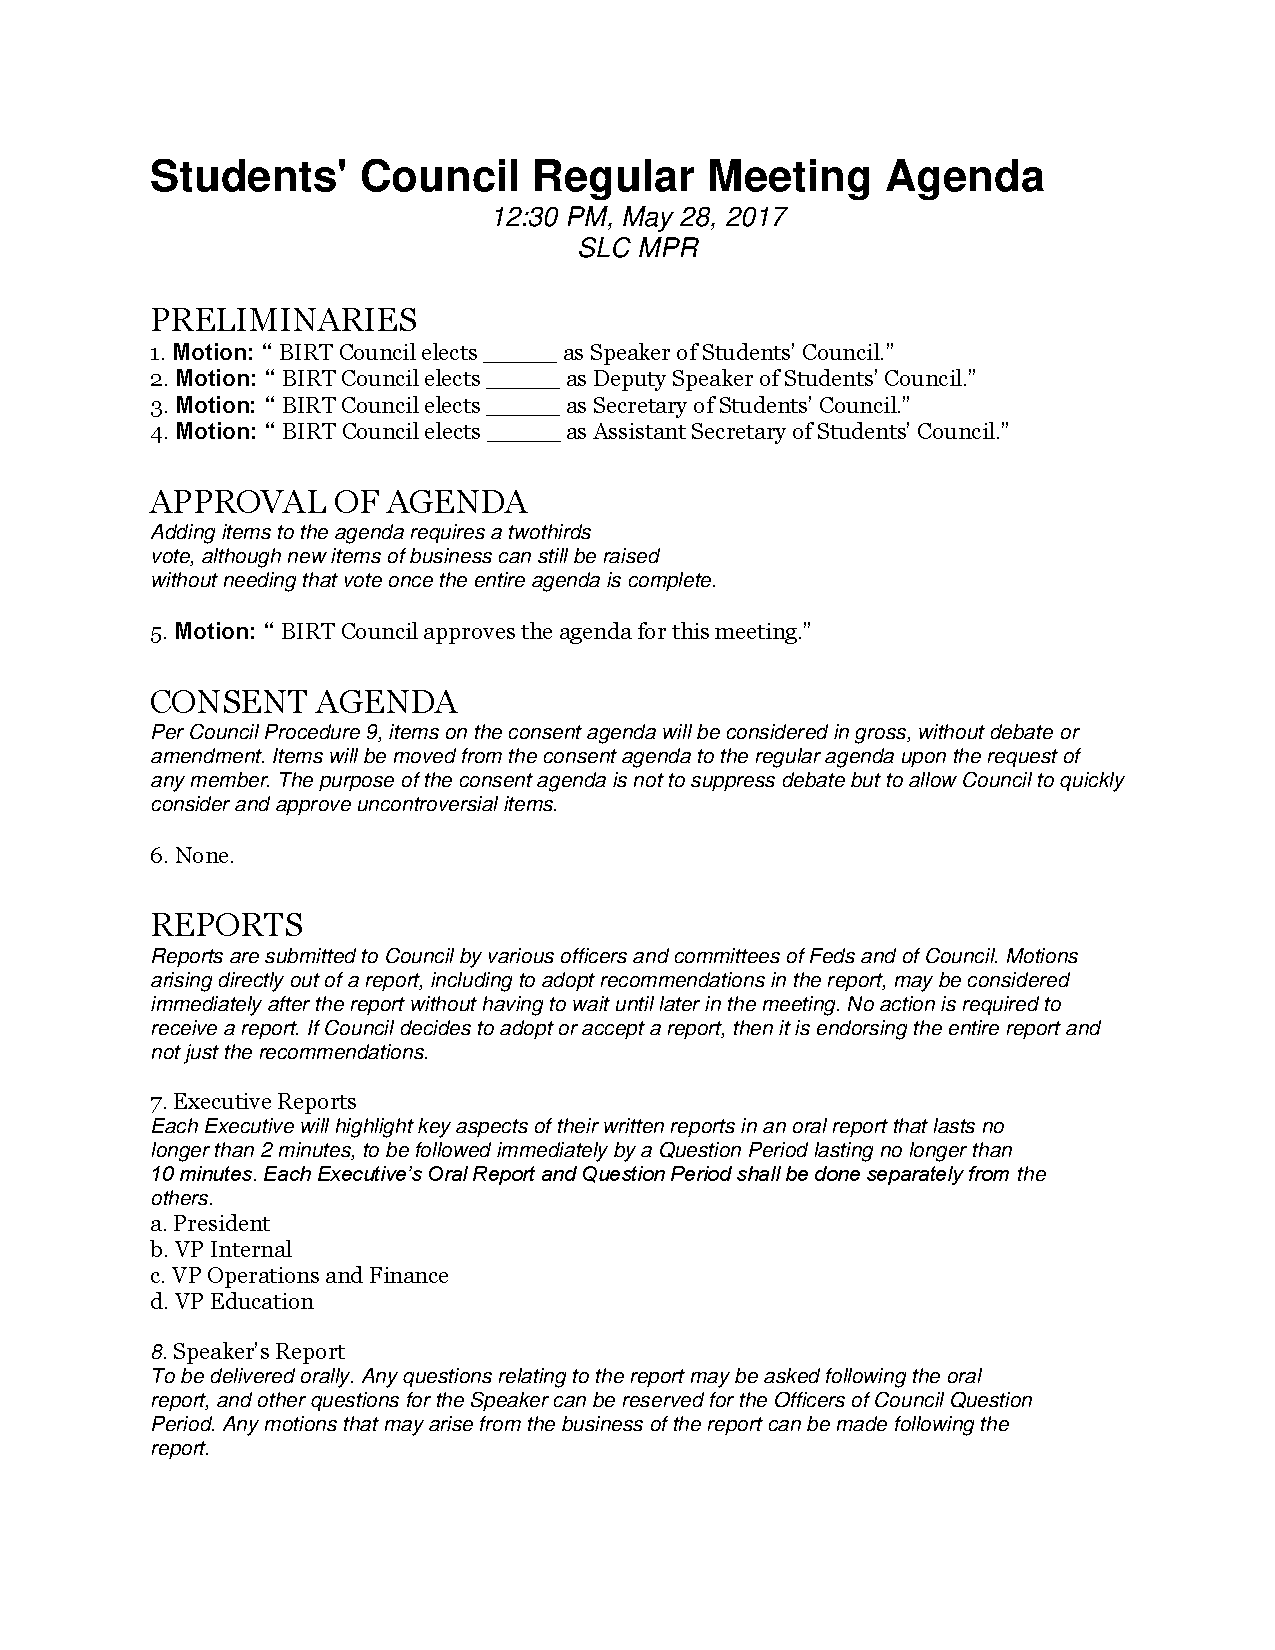
\includepdf[pages={-},scale=.8,pagecommand={}]{agenda/agenda.pdf}


\includepdf[pages={-},scale=.8,pagecommand={}]{agenda/reports/president.pdf}

\includepdf[pages={-},scale=.8,pagecommand={}]{agenda/reports/vped.pdf}

\includepdf[pages={-},scale=.8,pagecommand={}]{agenda/reports/vpi.pdf}
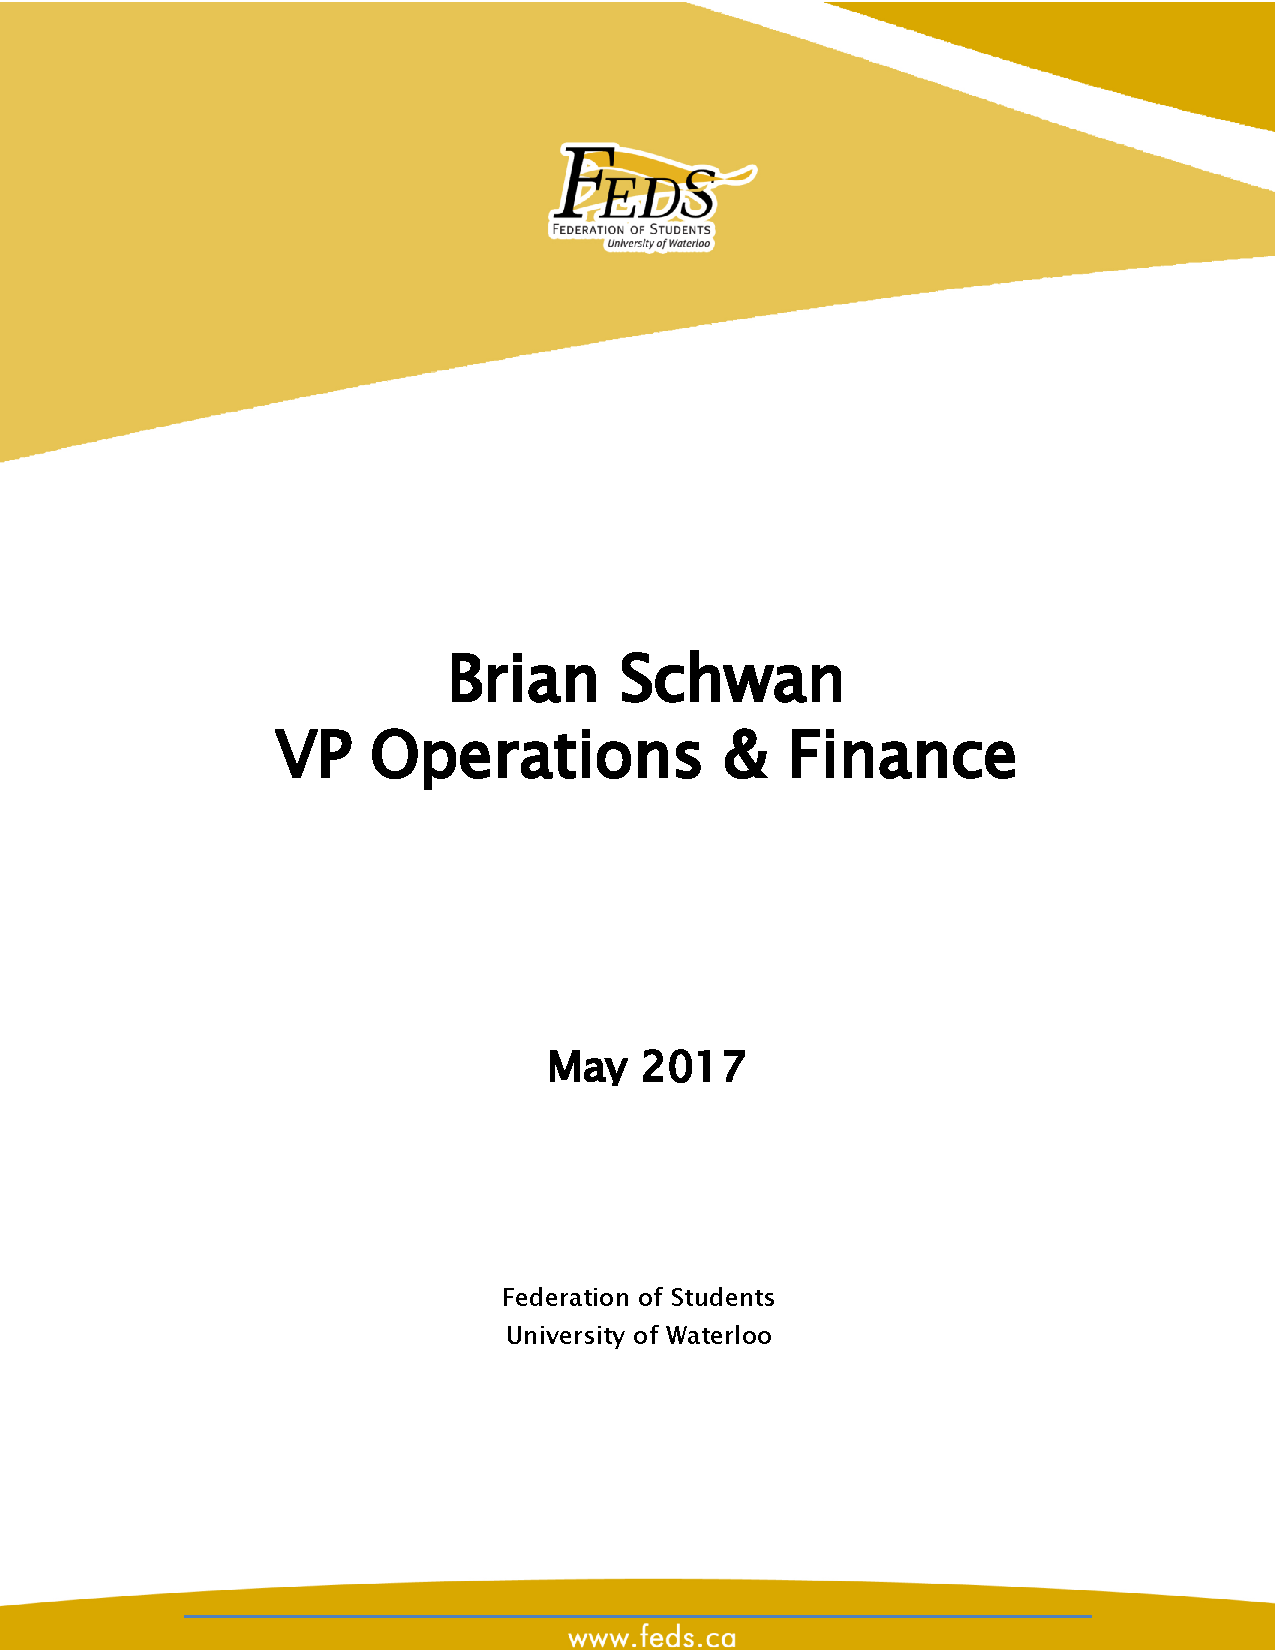
\includepdf[pages={-},scale=.8,pagecommand={}]{agenda/reports/vpof.pdf}


\includepdf[pages={-},scale=.8,pagecommand={}]{agenda/reports/bike-center.pdf}
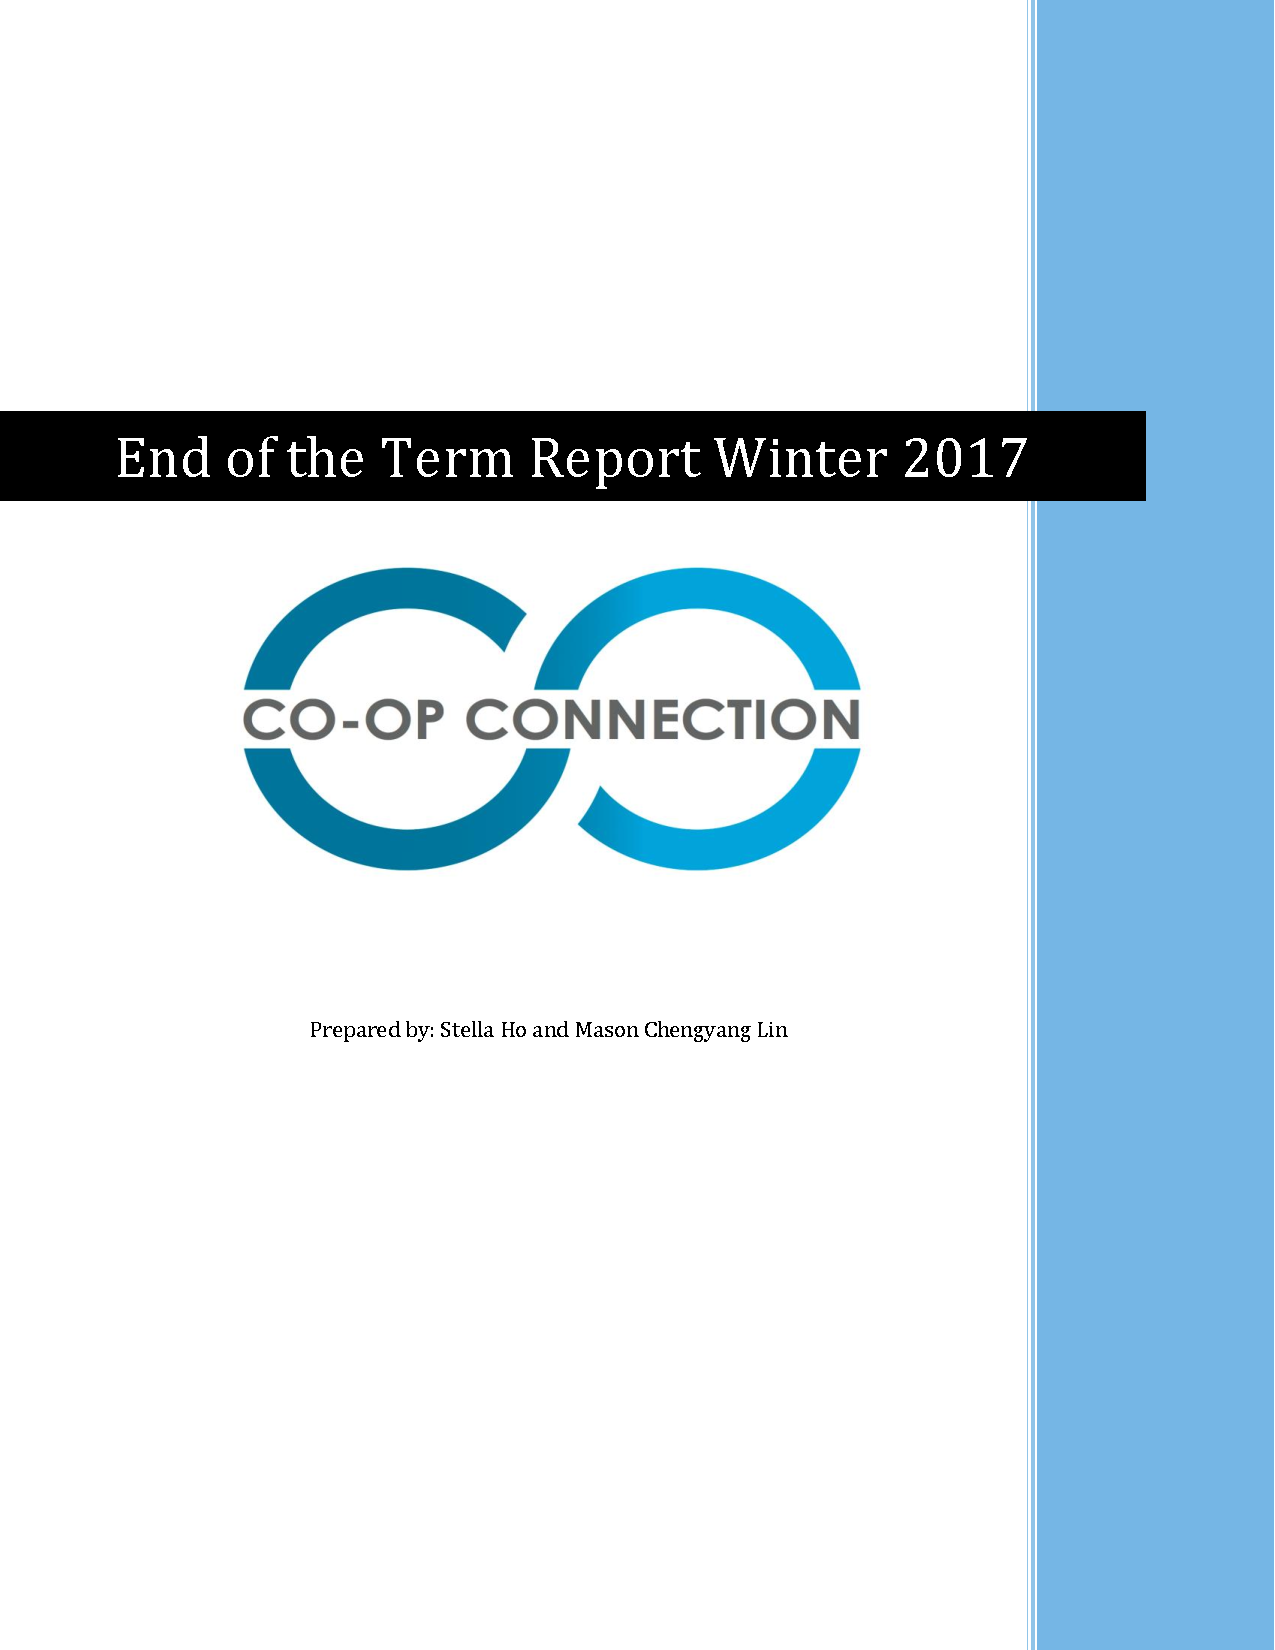
\includepdf[pages={-},scale=.8,pagecommand={}]{agenda/reports/coop-connection.pdf}

\includepdf[pages={-},scale=.8,pagecommand={}]{agenda/reports/crt.pdf}

\includepdf[pages={-},scale=.8,pagecommand={}]{agenda/reports/glow-centre.pdf}

\includepdf[pages={-},scale=.8,pagecommand={}]{agenda/reports/international-student-network.pdf}
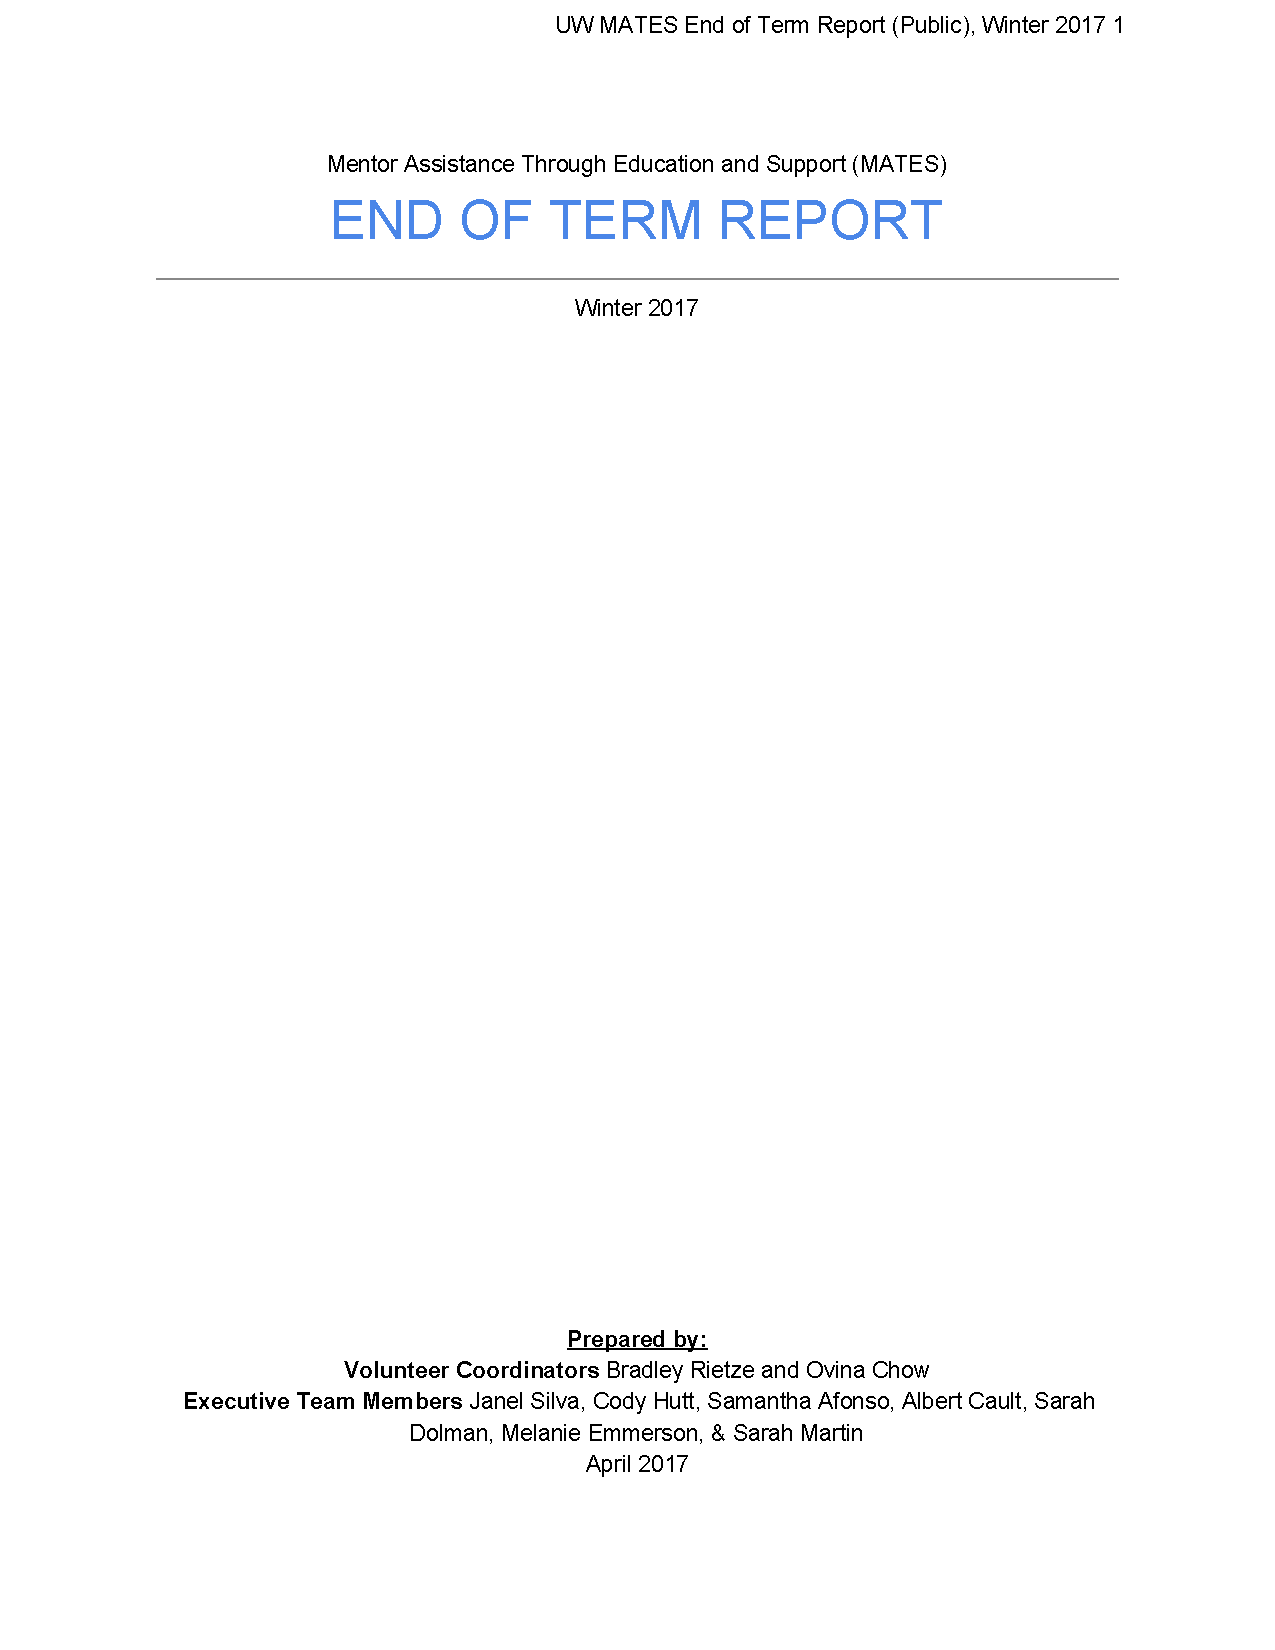
\includepdf[pages={-},scale=.8,pagecommand={}]{agenda/reports/mates.pdf}
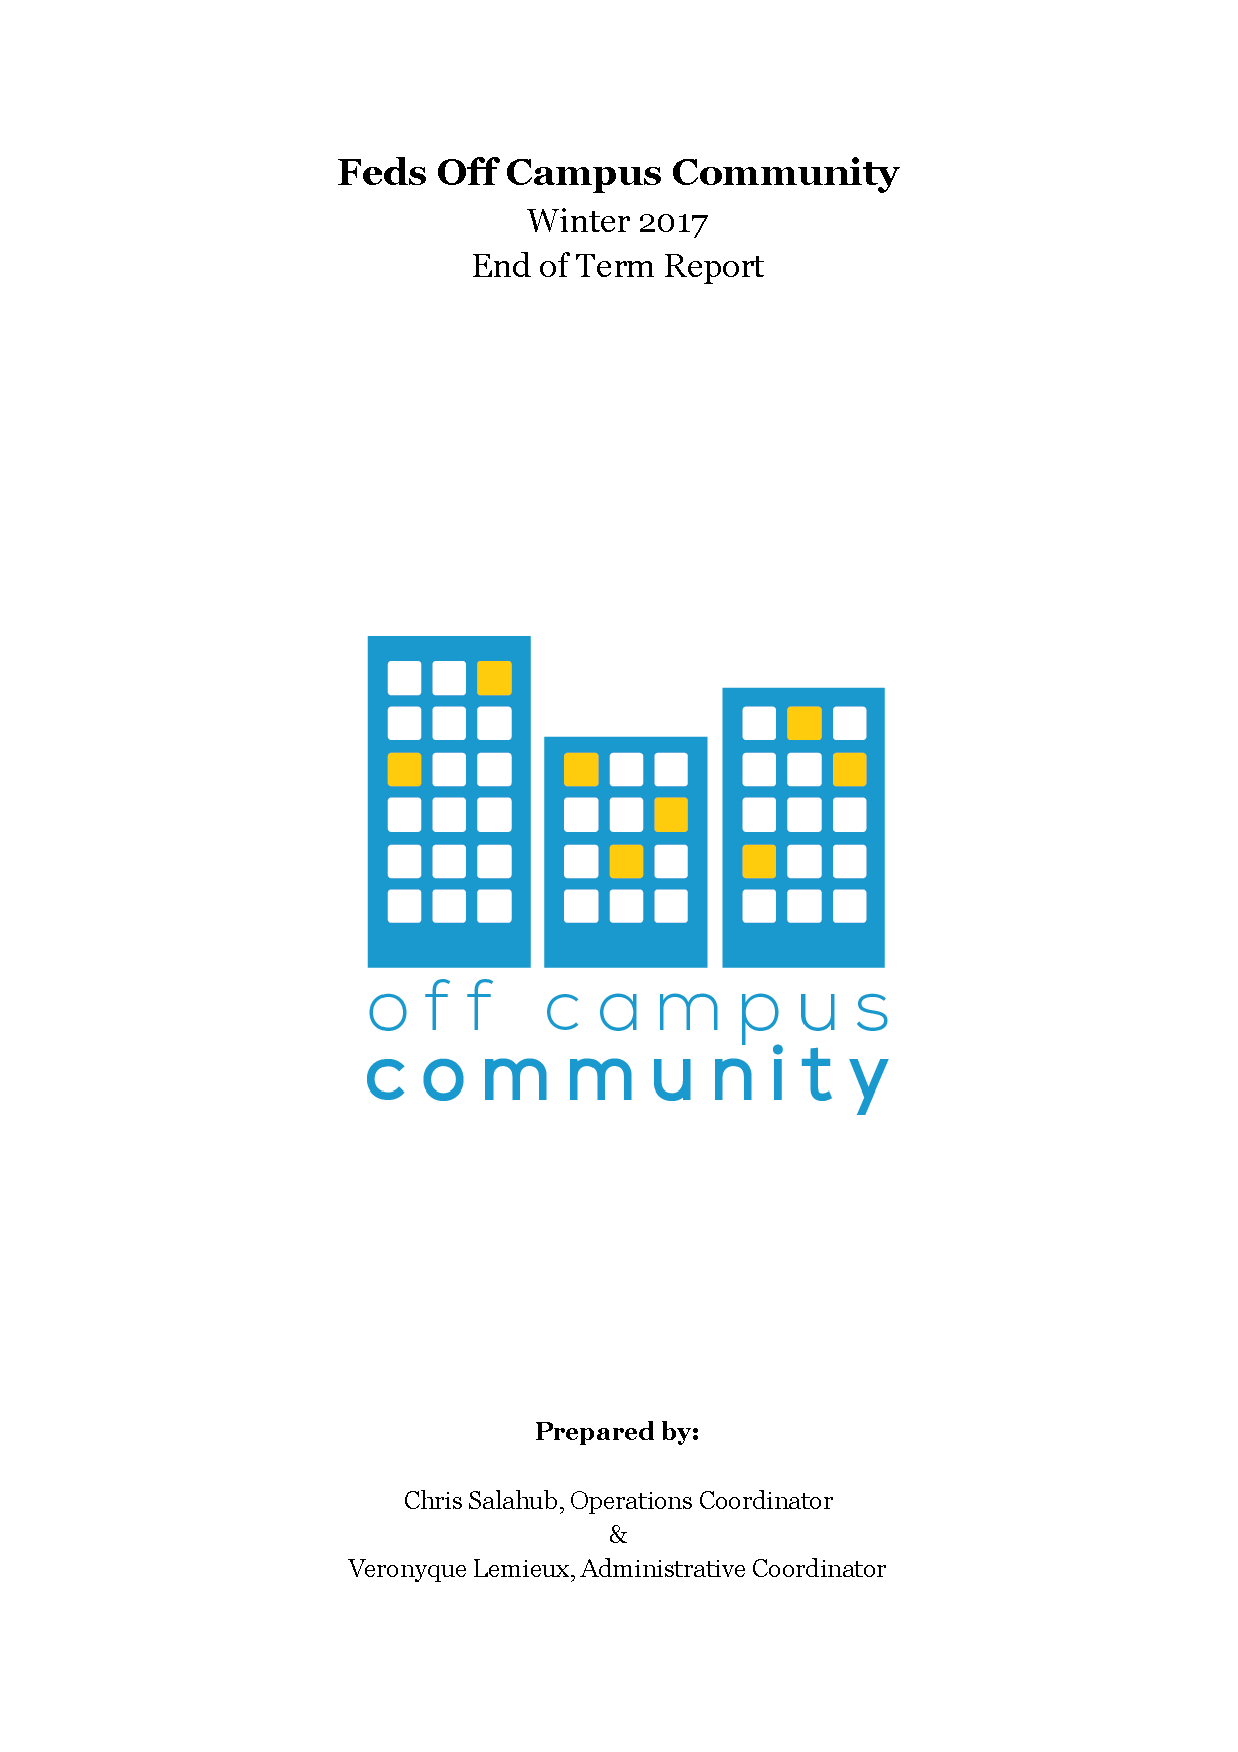
\includepdf[pages={-},scale=.8,pagecommand={}]{agenda/reports/off-campus-community.pdf}
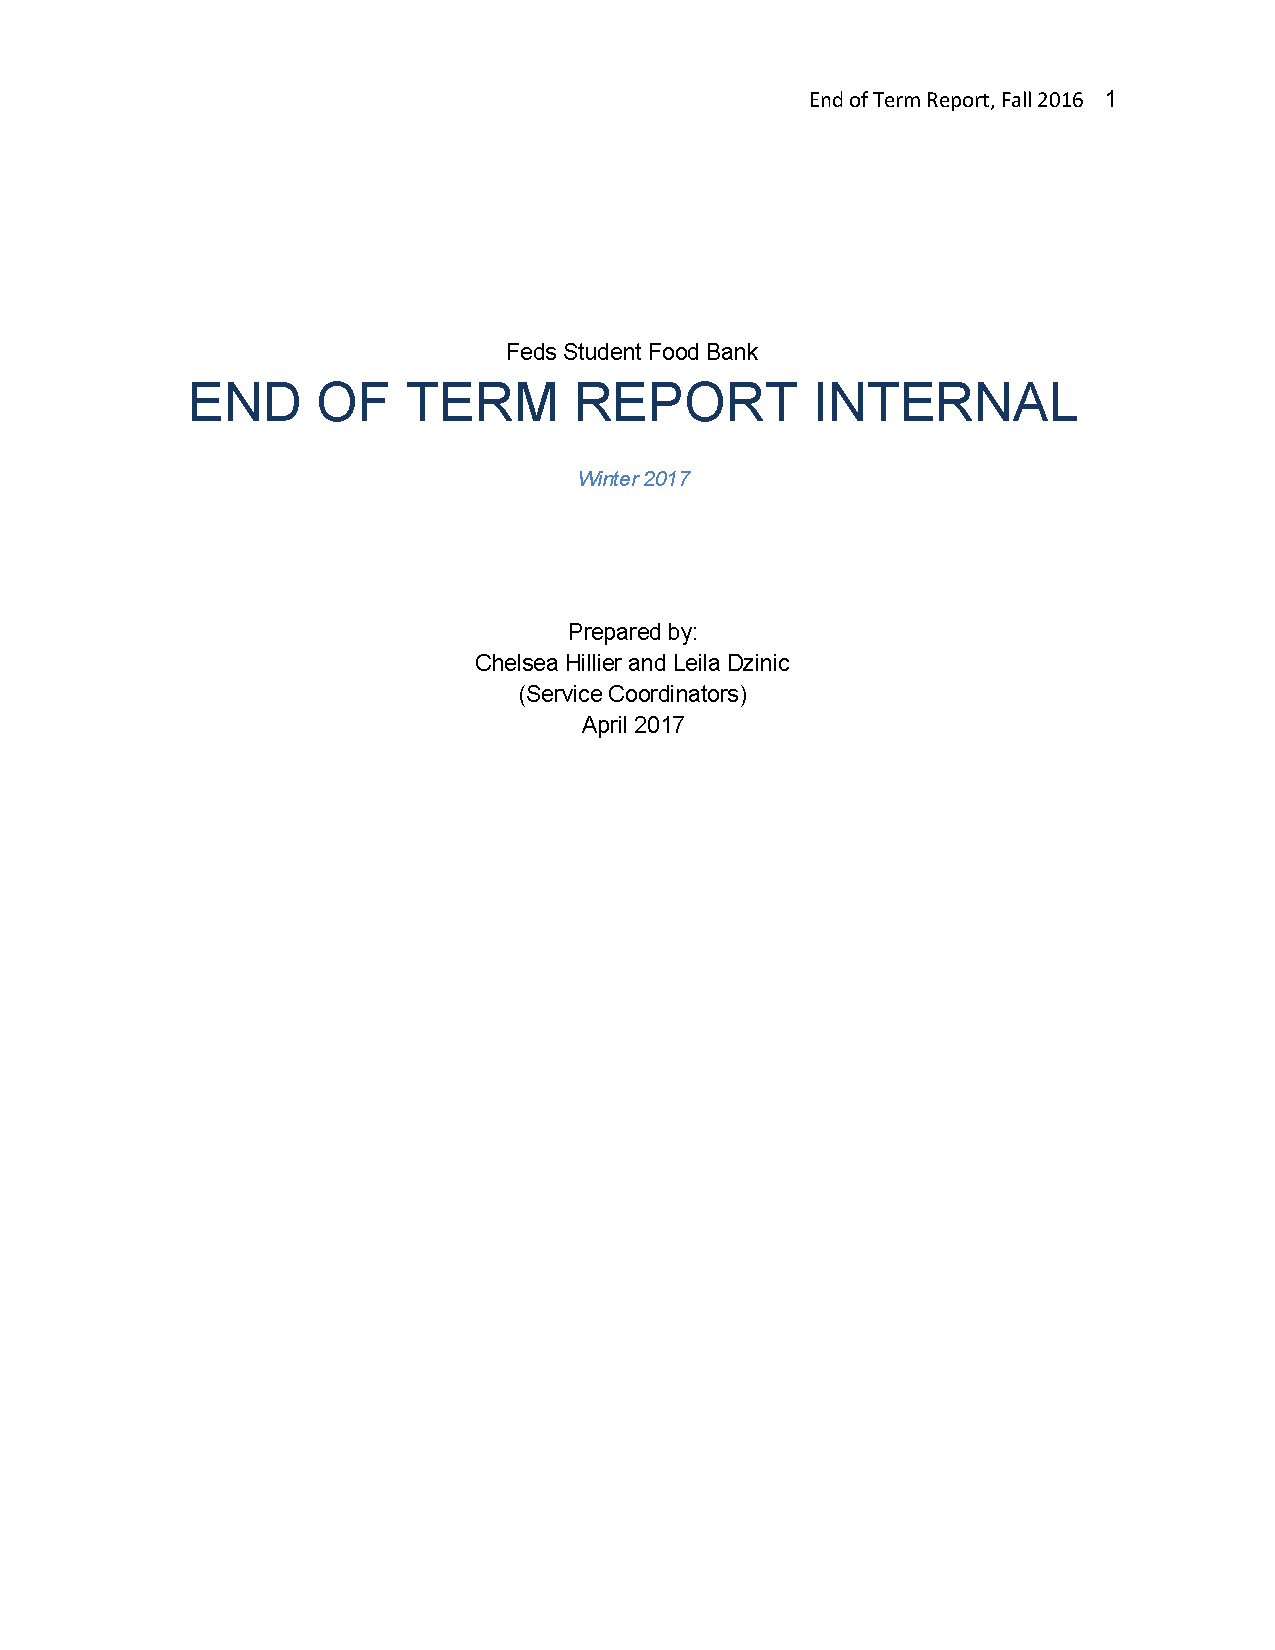
\includepdf[pages={-},scale=.8,pagecommand={}]{agenda/reports/student-food-bank.pdf}

\includepdf[pages={-},scale=.8,pagecommand={}]{agenda/reports/sustainable-campus.pdf}

\includepdf[pages={-},scale=.8,pagecommand={}]{agenda/reports/volunteer-centre.pdf}
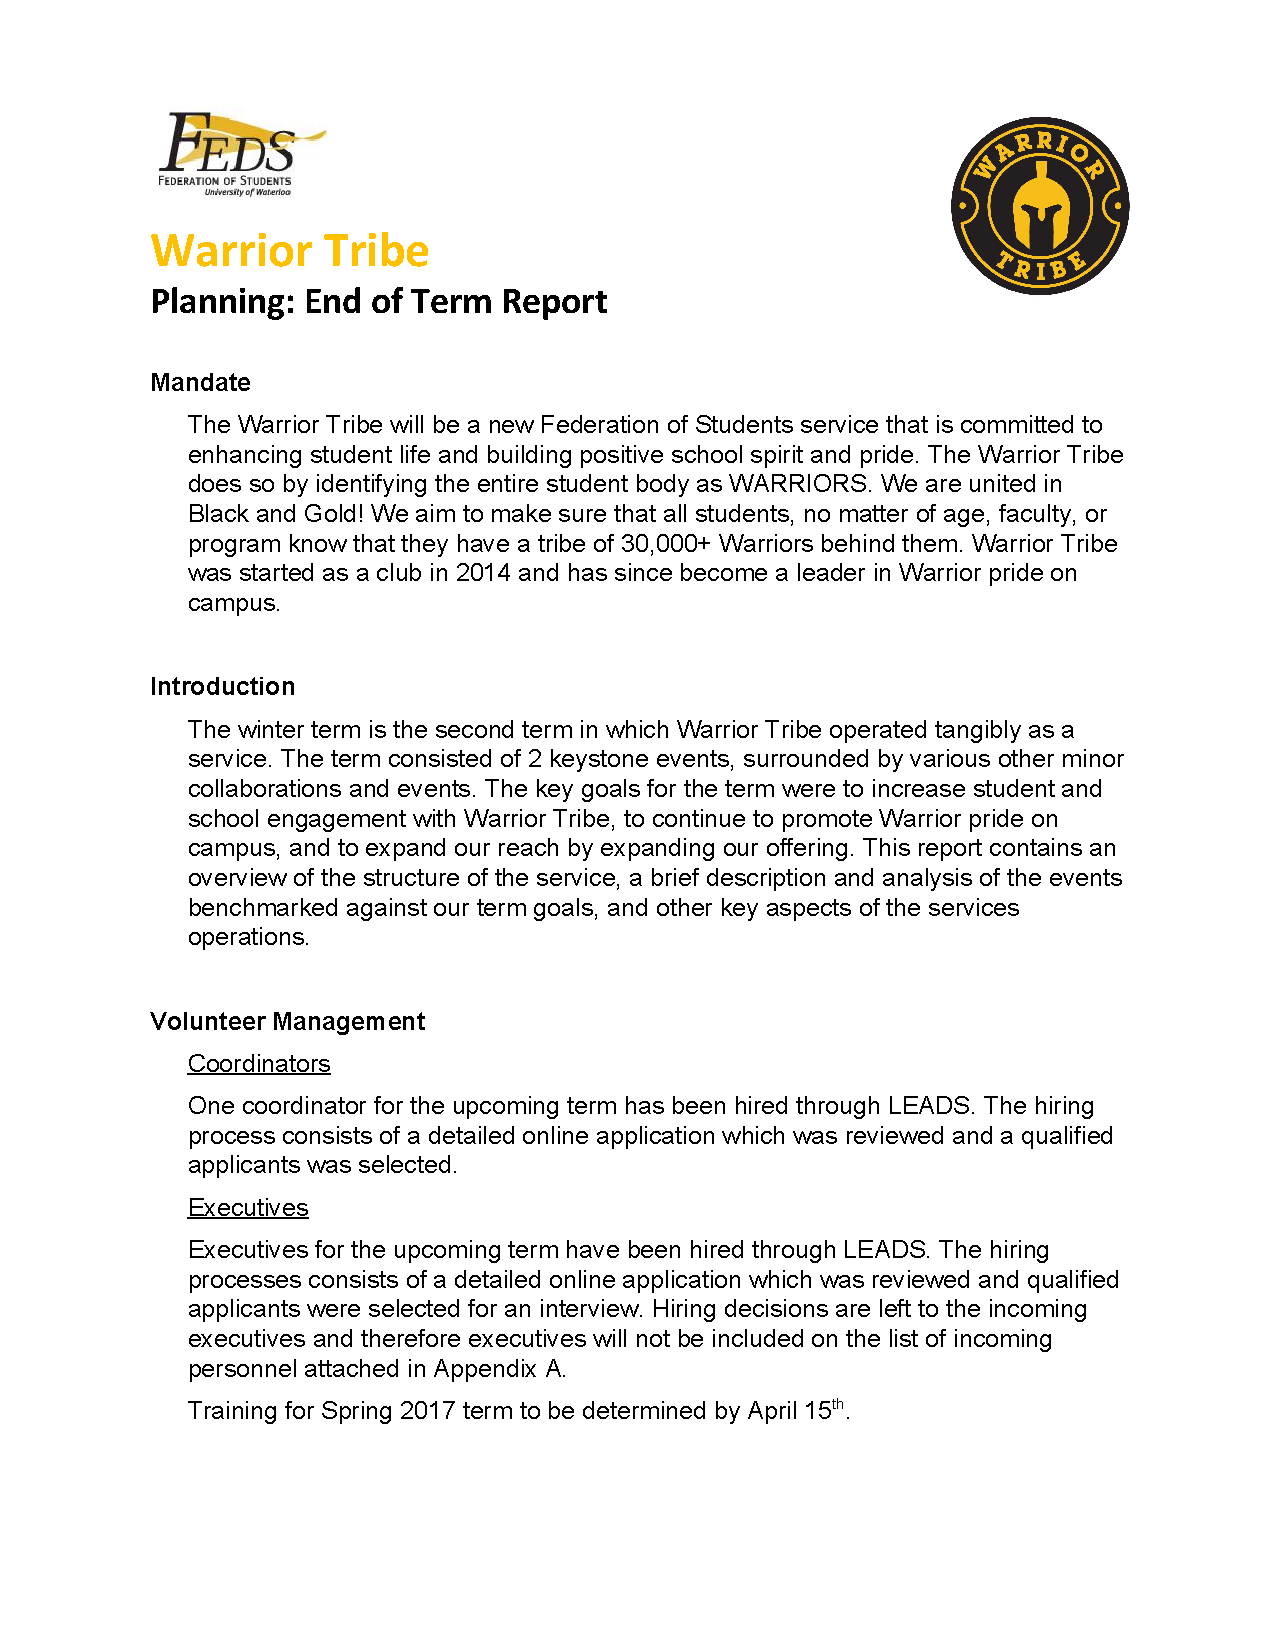
\includepdf[pages={-},scale=.8,pagecommand={}]{agenda/reports/warrior-tribe.pdf}
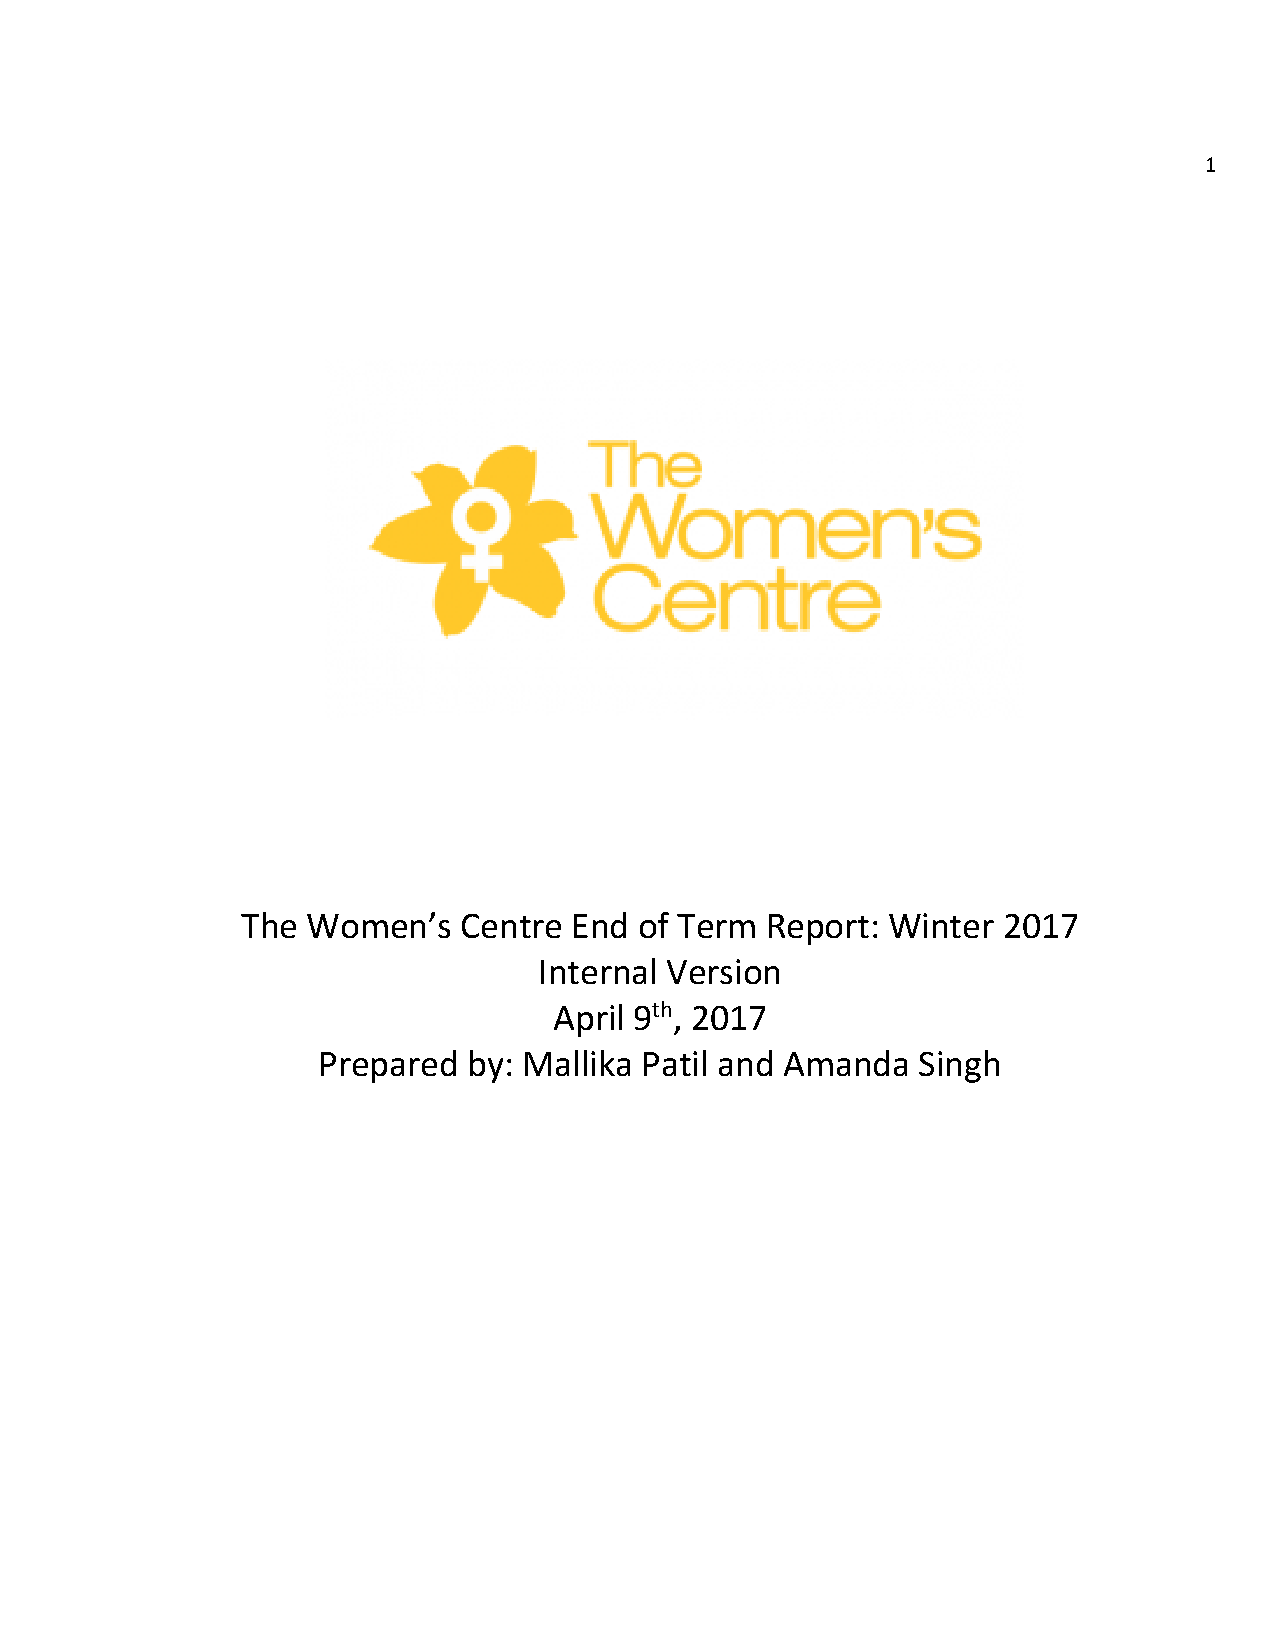
\includepdf[pages={-},scale=.8,pagecommand={}]{agenda/reports/womens-centre.pdf}

\end{document}
